% Target: Computer Vision Conference (CVC) 2027 -- Springer LNNS, llncs class.
% Main text limited to 6 pages excluding references; supporting material follows the bibliography.
% Every number is a macro generated from the raw predictions:
%   analysis/numbers.tex      <- Paper/analysis/analyze.py        (main experiment)
%   analysis/numbers_rev.tex  <- Revision1/a07_paper_assets.py    (robustness, detector, router)
% Do not type numbers by hand.
\documentclass[runningheads]{llncs}

\usepackage[T1]{fontenc}
\usepackage{graphicx}
\usepackage{booktabs}
\usepackage{amsmath}
\usepackage{amssymb}
\usepackage{xcolor}
\usepackage[hidelinks]{hyperref}
\usepackage{microtype}
\usepackage{float}
\setlength{\emergencystretch}{1em}

% Auto-generated by analysis/analyze.py -- do not edit by hand.
\newcommand{\accBOneAll}{41.3}
\newcommand{\ciBOneAll}{[39.6, 43.1]}
\newcommand{\accBOneRel}{37.9}
\newcommand{\ciBOneRel}{[34.5, 41.2]}
\newcommand{\accBOneNon}{42.6}
\newcommand{\ciBOneNon}{[40.5, 44.7]}
\newcommand{\accBTwoAll}{37.8}
\newcommand{\ciBTwoAll}{[36.1, 39.4]}
\newcommand{\accBTwoRel}{34.0}
\newcommand{\ciBTwoRel}{[30.8, 37.2]}
\newcommand{\accBTwoNon}{39.0}
\newcommand{\ciBTwoNon}{[36.9, 41.0]}
\newcommand{\accBThreeAll}{43.1}
\newcommand{\ciBThreeAll}{[41.3, 44.9]}
\newcommand{\accBThreeRel}{33.4}
\newcommand{\ciBThreeRel}{[30.2, 36.6]}
\newcommand{\accBThreeNon}{46.7}
\newcommand{\ciBThreeNon}{[44.5, 48.8]}
\newcommand{\accPropAll}{42.7}
\newcommand{\ciPropAll}{[41.0, 44.5]}
\newcommand{\accPropRel}{33.4}
\newcommand{\ciPropRel}{[30.1, 36.8]}
\newcommand{\accPropNon}{46.2}
\newcommand{\ciPropNon}{[44.1, 48.3]}
\newcommand{\nLoaded}{3,080}
\newcommand{\nScored}{2,983}
\newcommand{\nRel}{800}
\newcommand{\nNon}{2,123}
\newcommand{\dBPAll}{$-$0.4}
\newcommand{\dciBPAll}{[$-$1.2, +0.4]}
\newcommand{\pBPAll}{0.43}
\newcommand{\wBPAll}{74}
\newcommand{\lBPAll}{85}
\newcommand{\dBPRel}{+0.0}
\newcommand{\dciBPRel}{[$-$2.1, +2.1]}
\newcommand{\pBPRel}{1.00}
\newcommand{\wBPRel}{37}
\newcommand{\lBPRel}{37}
\newcommand{\dBPNon}{$-$0.5}
\newcommand{\dciBPNon}{[$-$1.3, +0.4]}
\newcommand{\pBPNon}{0.31}
\newcommand{\wBPNon}{35}
\newcommand{\lBPNon}{45}
\newcommand{\dOTAll}{+1.8}
\newcommand{\dciOTAll}{[+0.3, +3.3]}
\newcommand{\pOTAll}{0.02}
\newcommand{\wOTAll}{293}
\newcommand{\lOTAll}{240}
\newcommand{\dOTRel}{$-$4.5}
\newcommand{\dciOTRel}{[$-$7.5, $-$1.5]}
\newcommand{\pOTRel}{0.004}
\newcommand{\wOTRel}{56}
\newcommand{\lOTRel}{92}
\newcommand{\dOTNon}{+4.1}
\newcommand{\dciOTNon}{[+2.4, +5.9]}
\newcommand{\pOTNon}{9\times10^{-6}}
\newcommand{\wOTNon}{233}
\newcommand{\lOTNon}{146}
\newcommand{\dOTwAll}{$-$3.6}
\newcommand{\dciOTwAll}{[$-$5.4, $-$1.7]}
\newcommand{\pOTwAll}{2\times10^{-4}}
\newcommand{\wOTwAll}{333}
\newcommand{\lOTwAll}{439}
\newcommand{\dOTwRel}{$-$3.9}
\newcommand{\dciOTwRel}{[$-$7.2, $-$0.4]}
\newcommand{\pOTwRel}{0.04}
\newcommand{\wOTwRel}{87}
\newcommand{\lOTwRel}{118}
\newcommand{\dOTwNon}{$-$3.6}
\newcommand{\dciOTwNon}{[$-$5.7, $-$1.5]}
\newcommand{\pOTwNon}{0.001}
\newcommand{\wOTwNon}{236}
\newcommand{\lOTwNon}{313}
\newcommand{\dTwTAll}{+5.3}
\newcommand{\dciTwTAll}{[+3.5, +7.2]}
\newcommand{\pTwTAll}{3\times10^{-8}}
\newcommand{\wTwTAll}{486}
\newcommand{\lTwTAll}{327}
\newcommand{\dTwTRel}{$-$0.6}
\newcommand{\dciTwTRel}{[$-$4.1, +2.9]}
\newcommand{\pTwTRel}{0.78}
\newcommand{\wTwTRel}{104}
\newcommand{\lTwTRel}{109}
\newcommand{\dTwTNon}{+7.7}
\newcommand{\dciTwTNon}{[+5.5, +9.9]}
\newcommand{\pTwTNon}{1\times10^{-11}}
\newcommand{\wTwTNon}{374}
\newcommand{\lTwTNon}{210}
\newcommand{\didVal}{$-$8.6}
\newcommand{\didCI}{[$-$12.1, $-$5.1]}
\newcommand{\didP}{1\times10^{-4}}
\newcommand{\zeroObj}{66}
\newcommand{\zeroRel}{67}
\newcommand{\shareCross}{21}
\newcommand{\crossFrac}{19}
\newcommand{\meanObjAny}{16.3}
\newcommand{\meanRelAny}{59.3}
\newcommand{\tilesSel}{5.1}
\newcommand{\tilesTot}{93}
\newcommand{\nNoR}{2,063}
\newcommand{\dNoR}{$-$0.0}
\newcommand{\dciNoR}{[$-$0.8, +0.7]}
\newcommand{\pNoR}{1.00}
\newcommand{\chgNoR}{5.6}
\newcommand{\nNoRRel}{329}
\newcommand{\dNoRRel}{$-$1.5}
\newcommand{\dciNoRRel}{[$-$3.6, +0.6]}
\newcommand{\pNoRRel}{0.27}
\newcommand{\chgNoRRel}{7.9}
\newcommand{\nNoRNon}{1,709}
\newcommand{\dNoRNon}{+0.2}
\newcommand{\dciNoRNon}{[$-$0.6, +1.0]}
\newcommand{\pNoRNon}{0.78}
\newcommand{\chgNoRNon}{5.1}
\newcommand{\nHasR}{920}
\newcommand{\dHasR}{$-$1.1}
\newcommand{\dciHasR}{[$-$3.2, +1.0]}
\newcommand{\pHasR}{0.35}
\newcommand{\chgHasR}{17.4}
\newcommand{\nHasRRel}{471}
\newcommand{\dHasRRel}{+1.1}
\newcommand{\dciHasRRel}{[$-$2.1, +4.2]}
\newcommand{\pHasRRel}{0.61}
\newcommand{\chgHasRRel}{24.8}
\newcommand{\nHasRNon}{414}
\newcommand{\dHasRNon}{$-$3.1}
\newcommand{\dciHasRNon}{[$-$5.8, $-$0.5]}
\newcommand{\pHasRNon}{0.03}
\newcommand{\chgHasRNon}{9.9}
\newcommand{\nCross}{549}
\newcommand{\dCross}{$-$0.9}
\newcommand{\dciCross}{[$-$3.6, +1.8]}
\newcommand{\pCross}{0.61}
\newcommand{\chgCross}{19.3}
\newcommand{\nCrossRel}{247}
\newcommand{\dCrossRel}{+2.8}
\newcommand{\dciCrossRel}{[$-$2.0, +7.7]}
\newcommand{\pCrossRel}{0.32}
\newcommand{\chgCrossRel}{30.0}
\newcommand{\nCrossNon}{293}
\newcommand{\dCrossNon}{$-$4.1}
\newcommand{\dciCrossNon}{[$-$7.5, $-$1.0]}
\newcommand{\pCrossNon}{0.02}
\newcommand{\chgCrossNon}{10.9}
\newcommand{\orcAll}{51.2}
\newcommand{\orcRel}{44.9}
\newcommand{\orcNon}{53.6}
\newcommand{\callsBOne}{1.00}
\newcommand{\secBOne}{3.0}
\newcommand{\mpixBOne}{0.98}
\newcommand{\tokBOne}{1,403}
\newcommand{\gpuhBOne}{2.5}
\newcommand{\callsBTwo}{9.15}
\newcommand{\secBTwo}{5.0}
\newcommand{\mpixBTwo}{7.83}
\newcommand{\tokBTwo}{11,810}
\newcommand{\gpuhBTwo}{4.3}
\newcommand{\callsBThree}{6.10}
\newcommand{\secBThree}{16.8}
\newcommand{\mpixBThree}{7.53}
\newcommand{\tokBThree}{12,006}
\newcommand{\gpuhBThree}{14.3}
\newcommand{\callsProp}{6.10}
\newcommand{\secProp}{16.9}
\newcommand{\mpixProp}{7.53}
\newcommand{\tokProp}{12,455}
\newcommand{\gpuhProp}{14.4}
\newcommand{\gpuhTotal}{35.6}
\newcommand{\tokDiff}{448}
\newcommand{\osrBOne}{32.4}
\newcommand{\osrBTwo}{30.2}
\newcommand{\osrBThree}{27.2}
\newcommand{\osrProp}{26.2}
\newcommand{\osrD}{$-$5.2}
\newcommand{\osrDci}{[$-$9.0, $-$1.2]}
\newcommand{\osrP}{0.01}
\newcommand{\osrPholm}{0.12}
\newcommand{\colD}{+6.0}
\newcommand{\colPholm}{8\times10^{-4}}
\newcommand{\rawItems}{19,481}
\newcommand{\rawUnparsed}{1.6}
\newcommand{\dupRate}{10.7}
\newcommand{\crossMerges}{623}
\newcommand{\borderShare}{22}
\newcommand{\extSec}{13.0}
\newcommand{\extShare}{77}
\newcommand{\timeRatio}{5.6}
\newcommand{\peakVram}{18}
\newcommand{\nUnscOLU}{97}
\newcommand{\nHeld}{60}
\newcommand{\shareCpred}{38}
\newcommand{\stageOverview}{2.6}
\newcommand{\stageSelection}{0.3}
\newcommand{\stageFinal}{0.9}
\newcommand{\stageCrops}{0.0}
\newcommand{\stageGraph}{0.003}
\newcommand{\shareCmin}{37}
\newcommand{\shareCmax}{41}
\newcommand{\shareCgt}{27}

% Auto-generated by Revision1/a07_paper_assets.py -- do not edit
\newcommand{\nPartitions}{8}
\newcommand{\crossWorstP}{0.031}
\newcommand{\crossRangeLo}{$-$9.2}
\newcommand{\crossRangeHi}{$-$5.7}
\newcommand{\crossOSR}{$-$8.4}
\newcommand{\crossOSRci}{[$-$12.5, $-$4.2]}
\newcommand{\mdeAllRel}{3.0}
\newcommand{\mdeCrossRel}{6.9}
\newcommand{\routerAcc}{44.3}
\newcommand{\routerDelta}{+1.2}
\newcommand{\routerCI}{[+0.4, +2.0]}
\newcommand{\routerP}{0.0039}
\newcommand{\routerCalls}{4.76}
\newcommand{\routerSaving}{22}
\newcommand{\routerKwAcc}{43.6}
\newcommand{\routerKwDelta}{+0.4}
\newcommand{\routerKwP}{0.41}
\newcommand{\routerKwSaving}{30}
\newcommand{\oracleTwo}{51.2}
\newcommand{\selCalls}{6.10}
\newcommand{\routerFolds}{5}
\newcommand{\routerRepeats}{20}
\newcommand{\detN}{1,201}
\newcommand{\detNrel}{800}
\newcommand{\detNnon}{401}
\newcommand{\accDirAll}{41.2}
\newcommand{\accDirRel}{37.9}
\newcommand{\accDirNon}{47.9}
\newcommand{\accSelVAll}{38.6}
\newcommand{\accSelVRel}{33.4}
\newcommand{\accSelVNon}{48.9}
\newcommand{\accPropVAll}{38.0}
\newcommand{\accPropVRel}{33.4}
\newcommand{\accPropVNon}{47.1}
\newcommand{\accSelDAll}{36.7}
\newcommand{\accSelDRel}{31.5}
\newcommand{\accSelDNon}{47.1}
\newcommand{\accPropDAll}{38.4}
\newcommand{\accPropDRel}{33.2}
\newcommand{\accPropDNon}{48.6}
\newcommand{\relVAll}{$-$0.6}
\newcommand{\relVAllci}{[$-$2.1, +0.9]}
\newcommand{\relVAllp}{0.52}
\newcommand{\relVAllw}{40}
\newcommand{\relVAlll}{47}
\newcommand{\relDAll}{+1.7}
\newcommand{\relDAllci}{[$-$0.2, +3.5]}
\newcommand{\relDAllp}{0.095}
\newcommand{\relDAllw}{75}
\newcommand{\relDAlll}{55}
\newcommand{\impAll}{+2.2}
\newcommand{\impAllci}{[+0.0, +4.6]}
\newcommand{\impAllp}{0.07}
\newcommand{\relVRel}{+0.0}
\newcommand{\relVRelci}{[$-$2.1, +2.1]}
\newcommand{\relVRelp}{1}
\newcommand{\relVRelw}{37}
\newcommand{\relVRell}{37}
\newcommand{\relDRel}{+1.8}
\newcommand{\relDRelci}{[$-$0.6, +4.1]}
\newcommand{\relDRelp}{0.18}
\newcommand{\relDRelw}{54}
\newcommand{\relDRell}{40}
\newcommand{\impRel}{+1.8}
\newcommand{\impRelci}{[$-$1.2, +4.9]}
\newcommand{\impRelp}{0.29}
\newcommand{\relVNon}{$-$1.7}
\newcommand{\relVNonci}{[$-$3.5, +0.0]}
\newcommand{\relVNonp}{0.092}
\newcommand{\relVNonw}{3}
\newcommand{\relVNonl}{10}
\newcommand{\relDNon}{+1.5}
\newcommand{\relDNonci}{[$-$1.5, +4.5]}
\newcommand{\relDNonp}{0.41}
\newcommand{\relDNonw}{21}
\newcommand{\relDNonl}{15}
\newcommand{\impNon}{+3.2}
\newcommand{\impNonci}{[+0.0, +6.5]}
\newcommand{\impNonp}{0.066}
\newcommand{\detKwShare}{10}
\newcommand{\detTopLabel}{tree}
\newcommand{\detTopCount}{15,350}
\newcommand{\gVzero}{52}
\newcommand{\gDzero}{0}
\newcommand{\gVcross}{25}
\newcommand{\gDcross}{99}
\newcommand{\gVobj}{5.7}
\newcommand{\gDobj}{24.9}
\newcommand{\detObjOnly}{$-$1.8}
\newcommand{\detObjOnlyP}{0.067}
\newcommand{\detVsDirectRel}{$-$4.6}
\newcommand{\detVsDirectRelP}{0.0027}
\newcommand{\detGpuH}{4.2}

\graphicspath{{figures/}}

\newcommand{\pp}{\,pp}
\newcommand{\Bone}{\textit{Direct}}
\newcommand{\Btwo}{\textit{Tiling}}
\newcommand{\Bthree}{\textit{Selection}}
\newcommand{\Prop}{\textit{Proposed}}
\newcommand{\SelD}{\textit{Selection-D}}
\newcommand{\PropD}{\textit{Proposed-D}}

\begin{document}

\title{Resolution Without Relations: Quantifying the Perception--Reasoning Trade-off of Tile Selection in Ultra-High-Resolution Remote Sensing}
\titlerunning{Resolution Without Relations}

% TODO: author names and affiliations.
\author{Anonymous Author(s)}
\authorrunning{Anonymous}
\institute{Affiliation withheld for review}

\maketitle

\begin{abstract}
Vision-language models (VLMs) must downscale remote sensing scenes of ultra-high resolution (UHR), so a common remedy is to select tiles relevant to the question and reason over them at native resolution. We quantify what this costs and test whether it can be repaired. On \nLoaded{} XLRS-Bench items with Qwen2.5-VL-7B, under paired tests and a matched budget of VLM calls and encoded pixels, tile selection raises accuracy on perception questions by \dOTNon\pp{} but lowers it on relational questions by \dOTRel\pp{} (interaction \didVal\pp, $p<10^{-4}$), a crossover that holds under \nPartitions{} alternative definitions of the relational group. Supplying the missing layout explicitly, as a geometric graph of cross-tile relations, does not repair it (\dBPRel\pp, 95\% CI \dciBPRel). Replacing the VLM extractor with an object detector raises graph coverage from \gVcross\% to \gDcross\% of scenes and removes the harm the graph did to perception questions, but the relational gain remains small and not significant (\relDRel\pp{} \relDRelci). The diagnosis is relevance rather than availability: only \detKwShare\% of detected objects correspond to anything the question asks about. A cross-validated router that simply decides \emph{whether} to zoom is both more accurate than always zooming (\routerAcc\% vs \accBThreeAll\%, $p=\routerP$) and \routerSaving\% cheaper, which we argue is the better use of the budget today.
\keywords{Remote sensing \and Vision-language models \and Ultra-high resolution \and Spatial reasoning}
\end{abstract}

%-----------------------------------------------------------------------------
\section{Introduction}

UHR remote sensing images are 8,500$\times$8,500 pixels or larger. XLRS-Bench~\cite{wang2025xlrs} made plain what this means for VLMs: a target object may cover a few hundred pixels, and whole-image encoding~\cite{bai2025qwen25vl} downscales it away. The field's answer is to \emph{zoom}, by searching~\cite{wu2024vstar,shen2024zoomeye}, pruning tokens~\cite{luo2025lrsvqa}, retrieving regions~\cite{zhang2024imagerag}, or learning an active crop policy~\cite{liu2025zoomearth}. That zooming trades global context for local detail is increasingly recognised~\cite{tran2026lookbefore,wang2026beyondzooming}; what is missing is a measurement of the cost under a controlled budget, and a test of whether the lost context can simply be handed back to the model.

This paper provides both. We built the natural repair (Fig.~\ref{fig:pipeline}): objects extracted from the selected tiles are registered into one global pixel frame, deduplicated across tile seams, and turned into a geometric relation graph (direction, distance, adjacency, containment, intersection) that is appended to the final prompt. Before running the experiment we fixed the confirmatory hypothesis, that the graph would help relational sub-tasks and matter little elsewhere.

It did not. Our contributions are therefore a measurement, a negative result with its diagnosis, and a cheaper alternative:
\begin{itemize}
\item a \textbf{compute-accounted comparison of four methods} in which the two central ones run a single code path differing by one flag, with identical VLM calls and encoded pixels;
\item a \textbf{crossover}: zooming changes accuracy by \dOTNon\pp{} on perception and \dOTRel\pp{} on relational questions, robust to \nPartitions{} definitions of the relational group;
\item a \textbf{null for explicit relations that survives fixing its own main confound}: with an object detector supplying graphs on \gDcross\% of scenes, the relational gain is still only \relDRel\pp{} \relDRelci, and we trace this to object \emph{relevance} (\detKwShare\%), not availability;
\item a \textbf{router} that decides whether to zoom, outperforming always-zooming by \routerDelta\pp{} ($p=\routerP$) at \routerSaving\% fewer VLM calls.
\end{itemize}

%-----------------------------------------------------------------------------
\section{Related Work}

\textbf{High-resolution VLMs.} Tiling encoders such as Monkey~\cite{li2024monkey} and LLaVA-UHD~\cite{xu2024llavauhd}, and native dynamic-resolution models such as Qwen2.5-VL~\cite{bai2025qwen25vl}, raise the input pixel budget. Training-free methods add search or hierarchy at inference: V*~\cite{wu2024vstar}, ZoomEye~\cite{shen2024zoomeye} and DC$^2$~\cite{wang2025dc2}.
\textbf{UHR remote sensing.} XLRS-Bench~\cite{wang2025xlrs} and GeoLLaVA-8K~\cite{wang2025geollava8k} target 8K-scale scenes; LRS-VQA~\cite{luo2025lrsvqa} prunes tokens under text guidance, ImageRAG~\cite{zhang2024imagerag} retrieves regions, ZoomEarth~\cite{liu2025zoomearth} learns a zoom policy, and UHR-Micro~\cite{ni2026uhrmicro} documents a ``resolution illusion'' for small evidence.
\textbf{The resolution--context trade-off.} Concurrent work reports the same tension we measure: patch-based zooming recovers small targets but destroys global context, motivating adaptive routing between global and local views~\cite{tran2026lookbefore}, and a pilot on XLRS-Bench finds that zooming saturates on tasks needing global search or multi-region comparison~\cite{wang2026beyondzooming}. Our contribution is not the existence of this trade-off but its controlled quantification, an explicit test of the obvious repair, and the grounding diagnosis that explains why the repair fails.
\textbf{Structured intermediates.} VLMs are weak at spatial relations~\cite{chen2024spatialvlm,rahmanzadehgervi2024blind} and at coordinates given as text~\cite{cheng2024spatialrgpt}; scene graphs~\cite{johnson2015scenegraph} and visual programs~\cite{gupta2023visprog,suris2023vipergpt} externalise structure, while marks drawn on the image help where textual structure does not~\cite{yang2023som,izadi2025viser}. We test the textual form at UHR scale under matched compute and two grounding regimes.

%-----------------------------------------------------------------------------
\section{Method}

\begin{figure}[t]
\centering
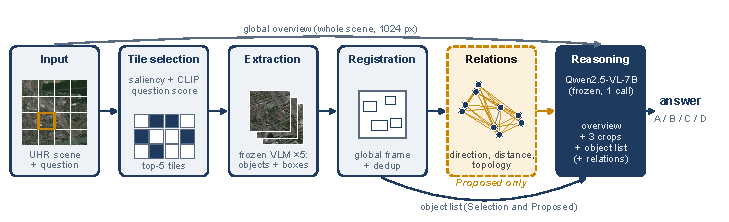
\includegraphics[width=\textwidth]{fig1_architecture.pdf}
\caption{The four compared methods; only the dashed relation block separates \Bthree{} from \Prop.}
\label{fig:pipeline}
\end{figure}

\textbf{Selection.} Each scene is cut into 1024-pixel tiles with 128 pixels of overlap (\tilesTot{} tiles per scene on average). Tiles are scored by $0.35\,s_\mathrm{sal}+0.65\,s_\mathrm{clip}$: gradient and variance energy on a downscaled overview, and CLIP~\cite{radford2021clip} similarity between the question and each tile thumbnail. The top-5 tiles are kept, suppressing near-duplicate neighbours.
\textbf{Local extraction and registration.} For each selected crop, the VLM returns JSON-formatted objects with boxes on a 0--1000 grid over the crop, which we lift to global pixels in code. Detections are merged across tiles by a label-aware greedy rule (IoU, containment, or near-touching boxes at a seam), yielding at most 60 objects per scene.
\textbf{Relations.} For each object and its 6 nearest neighbours we emit one predicate per pair, in priority order: containment (intersection over the smaller box $\geq$0.85); intersection (IoU $\geq$0.05 or overlap $\geq$5\% of the smaller box, e.g.\ roads crossing rivers); adjacency (border gap $\leq$1.2\% of the image diagonal); otherwise 8-way compass direction with pixel distance. At most 220 relations are kept, cross-tile edges first.
\textbf{Final call.} The final call receives the overview, 3 crops, and the object list in global 0--1000 coordinates. In \Prop{} it also receives the relation lines. The answer-format text is identical across methods. \Bone{} instead sends the whole image in a single call, and \Btwo{} answers on 8 grid tiles independently and reconciles them by a text-only vote; \Bthree{} and \Prop{} execute the same code path and issue $5{+}1$ calls over the same pixels, differing only in whether the relation block reaches the final prompt (Fig.~\ref{fig:pipeline}).

%-----------------------------------------------------------------------------
\section{Experimental Setup}

\textbf{Data.} We use the XLRS-Bench-lite split~\cite{wang2025xlrs}: \nLoaded{} four-option multiple-choice items (chance 25\%) in 13 categories. \nUnscOLU{} of the 100 Overall-Land-Use items are multi-select (e.g.\ answer ``BCD'') and were excluded from every method, leaving \nScored{} scored items. Before the experiment we fixed the relational group: object spatial relationship, regional counting, counting with complex reasoning, and route planning (\nRel{} items); the remaining \nNon{} items form the non-relational group. A \nHeld-item bi-temporal category not matched by our taxonomy is held out of both groups but counted overall.
\textbf{Models and budget.} All methods use Qwen2.5-VL-7B-Instruct~\cite{bai2025qwen25vl} in bf16 with greedy decoding and 1,280 visual tokens per image, on one NVIDIA L40S (\gpuhTotal{} GPU-hours for the main experiment, \detGpuH{} for the detector variant).
\textbf{Statistics.} All comparisons are paired on items, using McNemar's exact test~\cite{mcnemar1947} and 10,000-sample paired bootstrap intervals~\cite{efron1993bootstrap}; per-task tests are Holm-corrected~\cite{holm1979}. The two group-level \Bthree{}~vs~\Prop{} tests are confirmatory; all other analyses are exploratory and labelled as such. Throughout, MPix counts the pixels actually encoded by the vision tower, and significance markers in figures are $^{*}p<.05$, $^{**}p<.01$, $^{***}p<.001$.

%-----------------------------------------------------------------------------

\begin{table}[t]
\centering
\caption{Accuracy (\%) and cost per item on the \nScored{} scored items.}
\label{tab:main}
\setlength{\tabcolsep}{3.4pt}
\begin{tabular}{@{}lrrrrrrr@{}}
\toprule
Method & Calls & MPix & Tokens & s/item & Overall & Relational & Non-rel. \\
\midrule
Direct               & \callsBOne   & \mpixBOne   & \tokBOne   & \secBOne   & \accBOneAll   & \textbf{\accBOneRel} & \accBOneNon \\
Tiling               & \callsBTwo   & \mpixBTwo   & \tokBTwo   & \secBTwo   & \accBTwoAll   & \accBTwoRel   & \accBTwoNon \\
Selection            & \callsBThree & \mpixBThree & \tokBThree & \secBThree & \textbf{\accBThreeAll} & \accBThreeRel & \textbf{\accBThreeNon} \\
Proposed             & \callsProp   & \mpixProp   & \tokProp   & \secProp   & \accPropAll   & \accPropRel   & \accPropNon \\
\bottomrule
\end{tabular}
\end{table}

\begin{figure}[t]
\centering
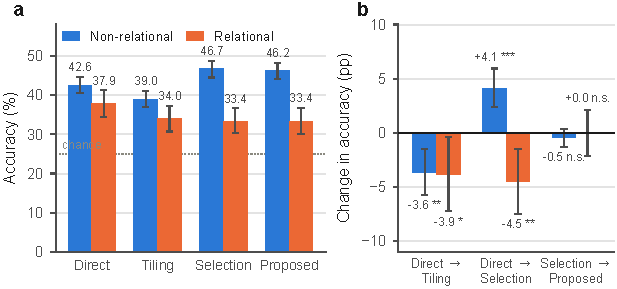
\includegraphics[width=\textwidth]{fig2_crossover.pdf}
\caption{Accuracy by method and task group (a), and paired changes with 95\% CIs (b).}
\label{fig:crossover}
\end{figure}

\section{Results}

\subsection{A crossover between perceptual and relational accuracy}
\Btwo{} is worse than \Bone{} in both groups (\dOTwAll\pp, $p=\pOTwAll$) despite 9$\times$ the calls: isolated crops lose scene context without adding structure. \Bthree{} recovers \dTwTNon\pp{} over \Btwo{} on non-relational tasks but nothing on relational ones (\dTwTRel\pp). Relative to \Bone, zooming therefore changes sign with the task group: \dOTNon\pp{} \dciOTNon{} for non-relational against \dOTRel\pp{} \dciOTRel{} for relational tasks, a difference of \didVal\pp{} \didCI{} (permutation $p<10^{-4}$, Fig.~\ref{fig:crossover}). On object spatial relationship (500 items) accuracy falls from \osrBOne\% with \Bone{} to \osrBThree\% with \Bthree, near the 25\% chance level.

This is not an artefact of our task grouping. Redefining the relational group \nPartitions{} ways, including the spatial-relationship task alone (\crossOSR\pp{} \crossOSRci) and the counting tasks alone, leaves the crossover between \crossRangeLo{} and \crossRangeHi\pp, significant in every case (worst $p=\crossWorstP$; Appendix~\ref{app:partitions}).

\subsection{Effect of explicit cross-tile relations}
Table~\ref{tab:main} gives the confirmatory result. On relational tasks \Prop{} and \Bthree{} score the same (\accPropRel\% each): \dBPRel\pp{} \dciBPRel{} ($p=\pBPRel$, \wBPRel{} wins against \lBPRel{} losses). On non-relational tasks the change is \dBPNon\pp{} \dciBPNon{} ($p=\pBPNon$). The two methods match in calls (\callsProp) and encoded pixels (\mpixProp{}~MP); the relation block adds \tokDiff{} prompt tokens and no measurable benefit. The interval excludes relational gains above \mdeAllRel\pp.

One explanation is mechanical: the VLM used as an object extractor returned nothing on \zeroObj\% of scenes here (98--100\% on object colour, classification and motion state), so the graph was usually empty and the test was partly a test of that emptiness.

\begin{figure}[t]
\centering
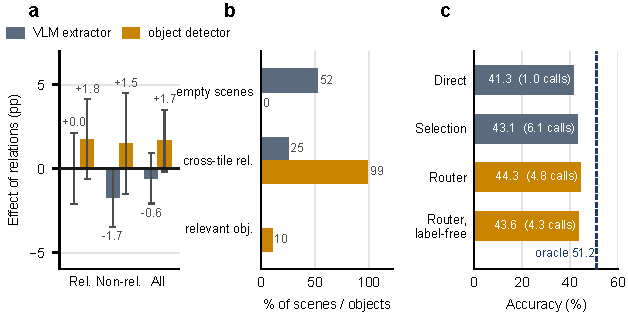
\includegraphics[width=\textwidth]{fig3_grounding_router.pdf}
\caption{Relation effect by grounding regime (a), extractor coverage (b), accuracy against cost (c).}
\label{fig:grounding}
\end{figure}

\subsection{Relation effects under detector-based grounding}\label{sec:detector}
We therefore replaced the extractor with a dedicated detector and repeated the comparison on \detN{} items (\detNrel{} relational, \detNnon{} non-relational), \emph{replaying the tiles each item received originally} so that only object extraction changes. The subset deliberately over-samples relational items, so its absolute accuracies are not comparable with Table~\ref{tab:main}; its paired effects are. The detector is Grounding DINO~\cite{liu2024groundingdino} (base checkpoint), an open-vocabulary transformer detector prompted with the question's keywords plus a fixed remote-sensing vocabulary (box threshold 0.30, text threshold 0.25, at most 24 boxes per tile). We call the resulting methods \SelD{} and \PropD.

Grounding improved sharply: scenes with no objects fell from \gVzero\% to \gDzero\%, those carrying a cross-tile relation rose from \gVcross\% to \gDcross\%, and objects per scene from \gVobj{} to \gDobj{} (Fig.~\ref{fig:grounding}b). The relation block nevertheless remains ineffective (Table~\ref{tab:detector}): \relDRel\pp{} \relDRelci{} on relational tasks ($p=\relDRelp$). What changes is its sign on perception questions, from \relVNon\pp{} to \relDNon\pp; pooled over all items, better grounding improves the relation effect by \impAll\pp{} \impAllci{} (permutation $p=\impAllp$), consistent in direction but short of significance.

\textbf{Availability is not relevance.} Only \detKwShare\% of the detector's objects match any content word of the question; its most frequent label is ``\detTopLabel'' (\detTopCount{} instances). Detector objects on their own are in fact slightly worse than the VLM's descriptions (\detObjOnly\pp, $p=\detObjOnlyP$), so a graph that is dense but generic does not help the model answer. The crossover also survives the change: \Bone{} still beats \PropD{} on relational items (\detVsDirectRel\pp, $p=\detVsDirectRelP$).

\begin{table}[t]
\centering
\caption{Accuracy (\%) and relation effects (pp, 95\% CI) under the two grounding regimes.}
\label{tab:detector}
\setlength{\tabcolsep}{4pt}
\begin{tabular}{@{}llrrr@{}}
\toprule
Objects from & Method & All & Relational & Non-rel. \\
\midrule
--                & Direct        & \accDirAll   & \accDirRel   & \accDirNon \\
VLM extractor     & Selection     & \accSelVAll  & \accSelVRel  & \accSelVNon \\
VLM extractor     & Proposed      & \accPropVAll & \accPropVRel & \accPropVNon \\
Detector          & Selection-D   & \accSelDAll  & \accSelDRel  & \accSelDNon \\
Detector          & Proposed-D    & \accPropDAll & \accPropDRel & \accPropDNon \\
\midrule
\multicolumn{2}{@{}l}{Relation effect, VLM extractor} & \relVAll{} \relVAllci & \relVRel{} \relVRelci & \relVNon{} \relVNonci \\
\multicolumn{2}{@{}l}{Relation effect, detector}      & \relDAll{} \relDAllci & \relDRel{} \relDRelci & \relDNon{} \relDNonci \\
\bottomrule
\end{tabular}
\end{table}

\subsection{Deciding when to zoom}
Back on all \nScored{} items, \Bone{} and \Bthree{} fail on different ones: an oracle choosing the better of the two per item reaches \oracleTwo\%, against \accBThreeAll\% for the best single method. We therefore learn a router with \routerFolds-fold cross-validation repeated \routerRepeats{} times, using only information available before answering, so no item's own outcome informs its routing. Routing on the task group reaches \routerAcc\%, exceeding \Bthree{} by \routerDelta\pp{} \routerCI{} ($p=\routerP$) while issuing \routerCalls{} VLM calls per item instead of \selCalls{} (\routerSaving\% fewer, Fig.~\ref{fig:grounding}c). Using only the question's keywords, without the benchmark's task label, the router matches \Bthree{} in accuracy (\routerKwAcc\%, $p=\routerKwP$) at \routerKwSaving\% fewer calls. Most of the oracle's headroom remains unclaimed, so better routing signals, not richer relation encodings, look like the productive direction.

%-----------------------------------------------------------------------------
\section{Discussion and Conclusion}

Under matched compute, explicit cross-tile relations did not improve UHR remote sensing VQA, and this held after we removed the obvious confound with a detector that supplied graphs on \gDcross\% of scenes. Three lessons follow. First, zoom-based pipelines trade relational for perceptual accuracy, so aggregate scores hide the trade and the two task families should be reported separately. Second, a symbolic relation layer is only as good as the \emph{relevance} of its grounding: dense but generic detections helped no more than sparse ones, which argues for query-conditioned detection rather than more predicates, and possibly for marks drawn on the image rather than text~\cite{izadi2025viser}. Third, the cheapest gain available today is not to zoom better but to decide when to zoom at all.
\textbf{Limitations:} one 7B model, the multiple-choice lite split only, one detector and one operating point, a generic CLIP scorer~\cite{liu2024remoteclip}, and a relational partition of our own design (Appendix~\ref{app:caveats}).
% TODO: add a code/data availability statement once a release location is decided.

\bibliographystyle{splncs04}
\bibliography{refs}

%=============================================================================
\clearpage
\appendix
\section{Supplementary Material}

\subsection{Robustness of the crossover to the relational partition}\label{app:partitions}
The crossover is the relational effect minus the non-relational one; the non-relational group is always the complement of the relational one, with the bi-temporal category excluded. $^{*}$ marks permutation $p<0.05$.
\begin{table}[H]
\centering
\caption{The crossover under alternative definitions of the relational group.}
\label{tab:partitions}
\setlength{\tabcolsep}{4pt}
\footnotesize
% Auto-generated by Revision1/a07_paper_assets.py
\begin{tabular}{@{}lrrrr@{}}
\toprule
Relational group & $n$ & Zoom, rel. & Zoom, non-rel. & Crossover [95\% CI] \\
\midrule
pre-registered & 800 & $-$4.5 & +4.1 & $-$8.6$^{*}$ [$-$12.0, $-$5.1] \\
spatial relationship only & 500 & $-$5.2 & +3.2 & $-$8.4$^{*}$ [$-$12.5, $-$4.2] \\
without counting tasks & 600 & $-$4.2 & +3.3 & $-$7.4$^{*}$ [$-$11.4, $-$3.5] \\
counting tasks only & 200 & $-$5.5 & +2.3 & $-$7.8$^{*}$ [$-$13.5, $-$2.1] \\
minus Counting with Complex Reasoning & 700 & $-$4.4 & +3.7 & $-$8.1$^{*}$ [$-$11.8, $-$4.5] \\
minus Object Spatial Relationship & 300 & $-$3.3 & +2.3 & $-$5.7$^{*}$ [$-$10.6, $-$0.8] \\
minus Regional Counting & 700 & $-$4.3 & +3.6 & $-$7.9$^{*}$ [$-$11.5, $-$4.3] \\
minus Route Planning & 700 & $-$5.3 & +4.0 & $-$9.2$^{*}$ [$-$12.9, $-$5.6] \\
\bottomrule
\end{tabular}

\end{table}

\subsection{Per-task results}
In Table~\ref{tab:pertask}, $\Delta_z$ is the change from \Bone{} to \Bthree{} and $\Delta_r$ the change from \Bthree{} to \Prop; Grp is R for relational, N for non-relational and H for the held-out category; the last column gives the share of scenes where the extractor returned no objects. Figure~\ref{fig:pertask} plots the same effects with 95\% CIs, slate for zooming and amber for the relation block, with $^{*}$ for Holm-adjusted $p<.05$; overall land use ($n{=}3$ scorable) is omitted and $^\dagger$ marks the held-out bi-temporal category.
\begin{table}[H]
\centering
\caption{Per-task accuracy (\%) and paired effects.}
\label{tab:pertask}
\setlength{\tabcolsep}{2.6pt}
\footnotesize
% Auto-generated by analysis/analyze.py
\begin{tabular}{@{}lcrrrrrrrr@{}}
\toprule
Task & Grp & $n$ & Direct & Tiling & Select. & Prop. & $\Delta_z$ & $\Delta_r$ & No obj. \\
\midrule
Complex counting & R & 100 & 56.0 & 43.0 & 51.0 & 52.0 & $-$5.0 & +1.0 & 48 \\
Object spatial rel. & R & 500 & 32.4 & 30.2 & 27.2 & 26.2 & $-$5.2 & $-$1.0 & 37 \\
Regional counting & R & 100 & 45.0 & 36.0 & 39.0 & 43.0 & $-$6.0 & +4.0 & 49 \\
Route planning & R & 100 & 40.0 & 42.0 & 41.0 & 41.0 & +1.0 & +0.0 & 28 \\
Anomaly detection & N & 100 & 70.0 & 65.0 & 70.0 & 65.0 & +0.0 & $-$5.0 & 14 \\
Environ. condition & N & 100 & 79.0 & 72.0 & 80.0 & 78.0 & +1.0 & $-$2.0 & 9 \\
Object class. & N & 800 & 35.0 & 31.5 & 37.9 & 38.6 & +2.9 & +0.8 & 98 \\
Object colour & N & 800 & 35.4 & 34.4 & 41.4 & 41.0 & +6.0$^{*}$ & $-$0.4 & 100 \\
Motion state & N & 60 & 65.0 & 65.0 & 66.7 & 66.7 & +1.7 & +0.0 & 100 \\
Overall counting & N & 60 & 25.0 & 16.7 & 33.3 & 26.7 & +8.3 & $-$6.7 & 13 \\
Overall land use & N & 3 & 66.7 & 66.7 & 66.7 & 66.7 & +0.0 & +0.0 & 0 \\
Regional land use & N & 200 & 68.0 & 56.0 & 72.5 & 71.5 & +4.5 & $-$1.0 & 11 \\
Bi-temporal counting & H & 60 & 43.3 & 46.7 & 46.7 & 45.0 & +3.3 & $-$1.7 & 40 \\
\bottomrule
\end{tabular}

\end{table}

\begin{figure}[H]
\centering
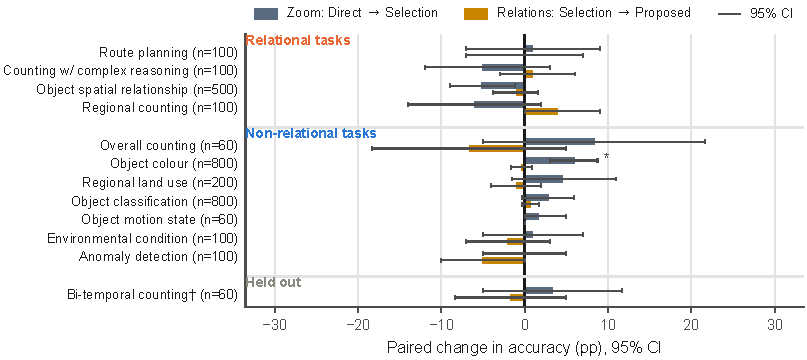
\includegraphics[width=\textwidth]{figA_per_task.pdf}
\caption{Paired per-task effects with 95\% CIs.}
\label{fig:pertask}
\end{figure}

\begin{figure}[H]
\centering
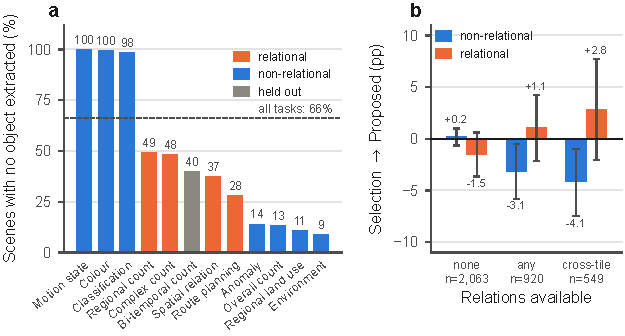
\includegraphics[width=\textwidth]{figA_mechanism.pdf}
\caption{Empty graphs per task (a), and the relation effect by what the graph contained (b).}
\label{fig:mechanism}
\end{figure}

Figure~\ref{fig:mechanism}a counts scenes in which the VLM extractor returned no object in any of the five selected crops. In Fig.~\ref{fig:mechanism}b the answer changed on \chgNoR\% of items when the block was empty, against \chgHasR\% and \chgCross\% when it carried any relation or a cross-tile relation, so the empty-block value is the noise floor from the prompt text alone.

\subsection{Further caveats}\label{app:caveats}
The planned ablation sweeps over tile size, overlap and top-$k$ were not run, so the configuration reported here is a single operating point. All methods chose option ``C'' for \shareCmin--\shareCmax\% of items, against \shareCgt\% of ground-truth answers: a position bias shared across methods, which affects absolute accuracy but not the paired comparisons. The \nUnscOLU{} multi-select Overall-Land-Use items were excluded identically from every method; set-based scoring of them is left to future work. Stratified analyses condition on the number of relations, a post-treatment variable, and their $p$-values are uncorrected. In the detector experiment, the relational gain on items carrying a cross-tile relation is detectable only above \mdeCrossRel\pp{} at 80\% power, so a small true effect cannot be excluded.

\subsection{Example inputs, questions and relation graph}\label{app:examples}
Figure~\ref{fig:input} shows one scene as the pipeline sees it, and Fig.~\ref{fig:graph} the relation graph built for it, in which 27 of the 32 relations connect objects observed in different tiles and \Prop{} answers correctly where \Bthree{} does not. Its labels also show a failure mode: the extractor copied the question's wording into its object labels. The qualitative pair at the end of this appendix contrasts that item with a regional land-use item where adding 116 relations turns a correct \Bthree{} answer into an error, relations acting as distractors on a perception task; dashed boxes are selected tiles and orange edges cross-tile relations. Table~\ref{tab:examples} lists real benchmark questions, verbatim.

\begin{figure}[H]
\centering
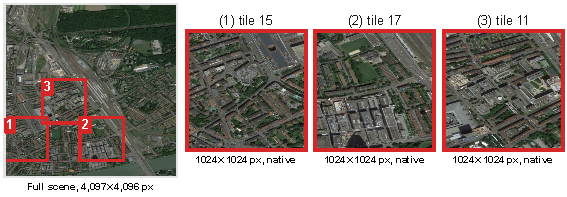
\includegraphics[width=\textwidth]{figA_input.pdf}
\caption{One scene as the pipeline sees it: selected tiles in context, then at native resolution.}
\label{fig:input}
\end{figure}

\begin{figure}[H]
\centering
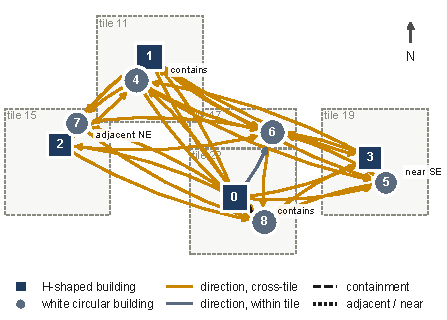
\includegraphics[width=0.8\textwidth]{figA_graph.pdf}
\caption{Relation graph for the scene in Fig.~\ref{fig:input}, with nodes at their global positions.}
\label{fig:graph}
\end{figure}

% Auto-generated by render_prompts.py -- verbatim XLRS-Bench-lite items
\begin{table}[H]
\centering
\caption{Example XLRS-Bench questions (verbatim). R marks tasks in the relational group, N the non-relational group.}
\label{tab:examples}
\scriptsize
\setlength{\tabcolsep}{3pt}
\begin{tabular}{@{}p{0.22\linewidth}c p{0.70\linewidth}@{}}
\toprule
Task & Grp & Question (answer) \\
\midrule
Counting with Complex Reasoning & R & How many parking lots are there in the town shown in the picture above? \emph{(D: 9)} \\
Object Spatial Relationship & R & In the image, the two smaller green rectangular greenhouses located towards the upper right are positioned in which direction relative to the larger multi-unit residential area? \emph{(C: To the right)} \\
Regional Counting & R & How many houses are there inside the red circle? \emph{(B: 5)} \\
Route Planning & R & In the image below, what is the shortest driving route from the building with the red pyramid roof to the parking lot at the port on the left? \emph{(B: Exit the building and head west. Continue straight through the first intersection. At the next intersection, turn left to reach your destination.)} \\
Anomaly Detection and Interpretation & N & The width and calmness of the river in the picture suggest? \emph{(D: It may serve as a vital natural water source, crucial for the surrounding ecosystem.)} \\
Object Classification & N & Identify the object category within the given bounding box in the satellite or aerial image. Image resolution: 4096 x 4097. Bounding box: [2368, 2061, 2447, 2108]. \emph{(B: The Red Roof)} \\
Object Color & N & Determine the color of the object within the given reference bounding box in the satellite image. Image resolution: 5616 x 3744. Bounding box: [3826, 1648, 3944, 1695]. \emph{(C: White)} \\
Overall Land Use Classification & N & Select the options that best represent the types of land use depicted in the image. \emph{(ABD: Farmland; Lakes or Ponds; Parking Lot or Garage [multi-select])} \\
Regional Land Use Classification & N & Select the type of land marked with a red circle in the image. \emph{(D: Farmland)} \\
\bottomrule
\end{tabular}
\end{table}


\subsection{Compute and extraction details}\label{app:compute}
Only \rawUnparsed\% of the \rawItems{} items returned by the VLM extractor lacked a readable box, so the empty graphs reflect the extractor returning no objects rather than malformed output. Mean seconds per item for \Prop: overview \stageOverview, selection \stageSelection, local extraction \extSec, final answer \stageFinal; deduplication and relation construction together take \stageGraph. Peak VRAM was \peakVram{}~GB. Deduplication merged \dupRate\% of raw detections, \crossMerges{} of them across tile seams, and \borderShare\% of parsed detections touched a tile border. The detector variant needs one VLM call per item instead of six, so its two runs together cost \detGpuH{} GPU-hours.

\subsection{Object count is confounded with task composition}
All methods improve together with the number of objects extracted, including \Bone, which never receives objects, so the trend reflects the mix of scenes and tasks per bin (labelled in Fig.~\ref{fig:confound}) rather than any benefit of the relation graph.
\begin{figure}[H]
\centering
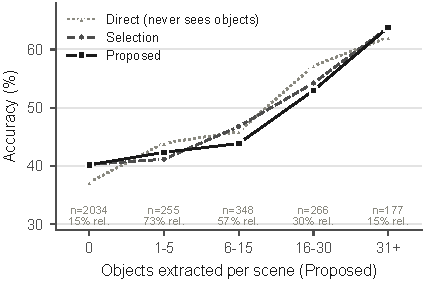
\includegraphics[width=0.66\textwidth]{figA_objects_confound.pdf}
\caption{Accuracy against the number of objects extracted, by method.}
\label{fig:confound}
\end{figure}

\subsection{Qualitative examples}
\begin{figure}[H]
\centering
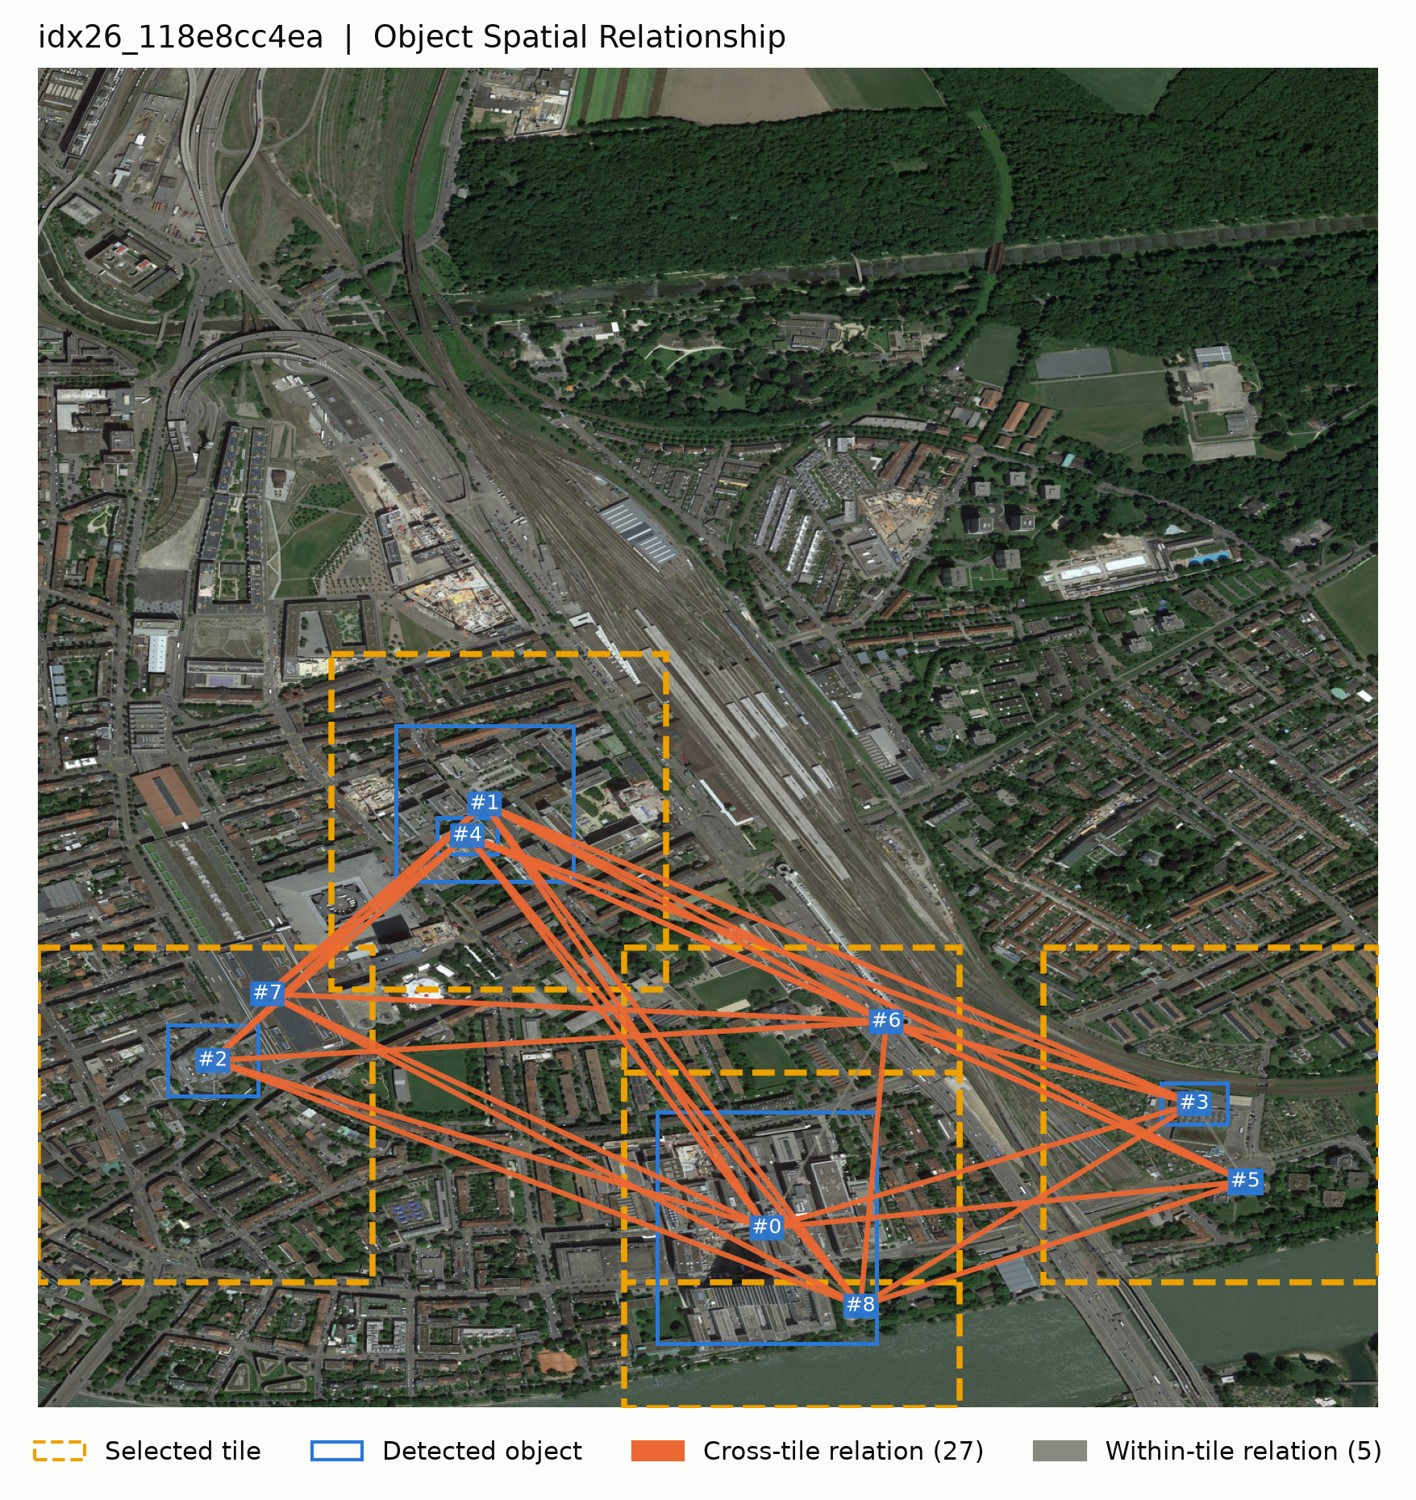
\includegraphics[width=0.49\textwidth]{figA_qual_win.jpg}\hfill
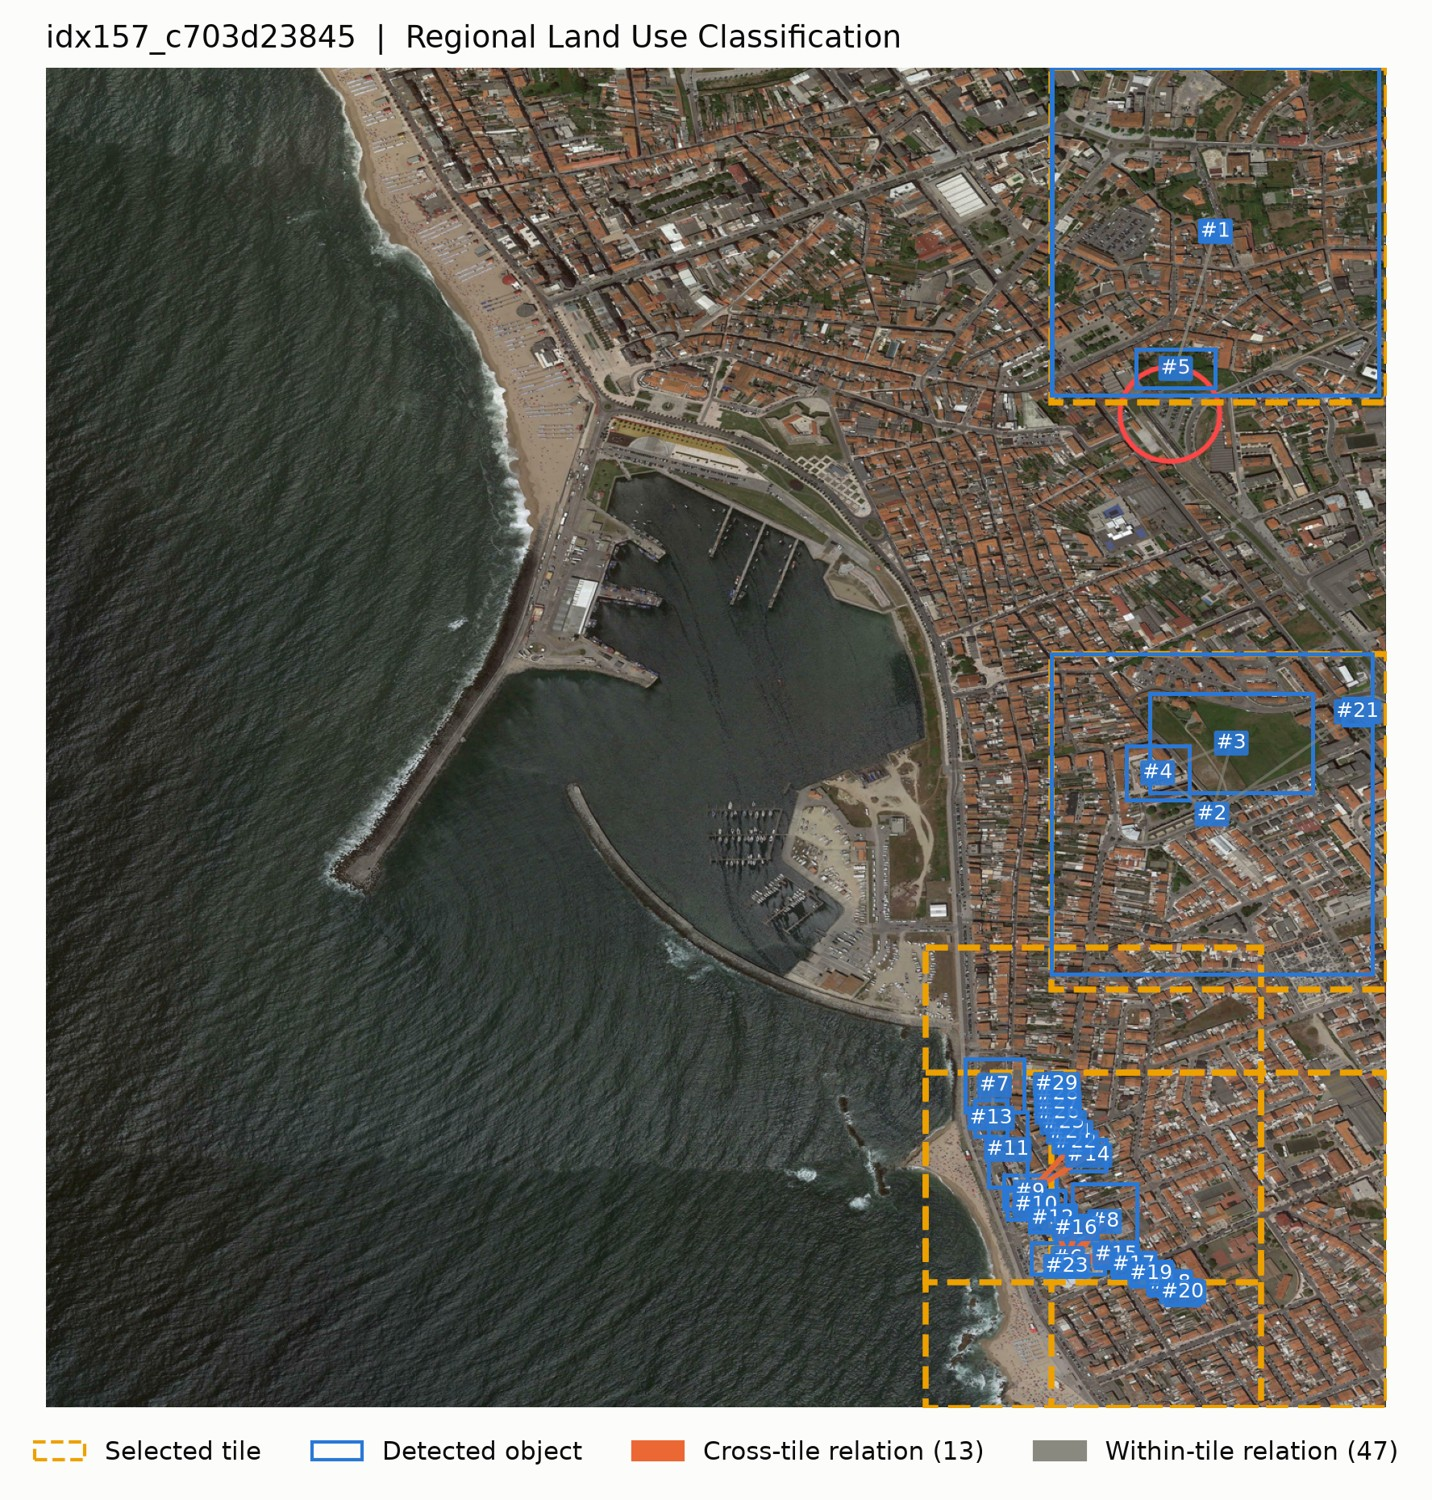
\includegraphics[width=0.49\textwidth]{figA_qual_loss.jpg}
\caption{A relational item the graph fixes (left) and a perception item it breaks (right).}
\end{figure}

\end{document}
